%%%%%%%%%%%%%%%%%%%%%%%%%%%%%%%%%%%%
% Slide options
%%%%%%%%%%%%%%%%%%%%%%%%%%%%%%%%%%%%

% Option 1: Slides with solutions

\documentclass[slidestop,compress,mathserif]{beamer}
\newcommand{\soln}[1]{\textit{#1}}
\newcommand{\solnGr}[1]{#1}

% Option 2: Handouts without solutions

%\documentclass[11pt,containsverbatim,handout]{beamer}
%\usepackage{pgfpages}
%\pgfpagesuselayout{4 on 1}[letterpaper,landscape,border shrink=5mm]
%\newcommand{\soln}[1]{ }
%\newcommand{\solnGr}{ }

%%%%%%%%%%%%%%%%%%%%%%%%%%%%%%%%%%%%
% Style
%%%%%%%%%%%%%%%%%%%%%%%%%%%%%%%%%%%%
%%%%%%%%%%%%%%%%%%%%%%%%%%%%%%%%%%%%%%%%%%%%%%%%%%%%%%%%%%%%%%%%%%%%%%%%
% MA213/214 shared slide style
%
% "Calm & Cool" palette + content-type callout boxes.
% Overhauled (2026) from the original OpenIntro/metropolis style:
%   - all OpenIntro visual branding removed (logo, grid, colors)
%   - a low-key cool palette (see colors below)
%   - tcolorbox callout boxes so students recognize content types
% See common/README.md for the command cheat-sheet.
%%%%%%%%%%%%%%%%%%%%%%%%%%%%%%%%%%%%%%%%%%%%%%%%%%%%%%%%%%%%%%%%%%%%%%%%

\usetheme{metropolis}

%%%%%%%%%%%%%%%%
% Packages
%%%%%%%%%%%%%%%%

\usepackage{geometry}
\usepackage{graphicx}
\usepackage{amssymb}
\usepackage{epstopdf}
\usepackage{amsmath}  	% this permits text in eqnarray among other benefits
\usepackage{url}		% produces hyperlinks
\usepackage{hyperref}	% allows for color usage in tables
\usepackage[english]{babel}
\usepackage[latin1]{inputenc}
\usepackage{colortbl}	% allows for color usage in tables
\usepackage{multirow}	% allows for rows that span multiple rows in tables
\usepackage{color}		% this package has a variety of color options
\usepackage{pgf}
\usepackage{calc}
\usepackage{ulem}
\usepackage{multicol}
\usepackage{textcomp}
\usepackage{txfonts}
\usepackage{listings}
\usepackage{tikz}
\usepackage{array}
\usepackage{wasysym}
\usepackage{fancyvrb}
\usepackage{etoolbox}             % \ifstrempty for optional box subtitles
\usepackage[most]{tcolorbox}      % content-type callout boxes
\tcbuselibrary{listings}          % R-code block (\begin{rblock})
\usepackage{fontawesome5}         % box icons

%%%%%%%%%%%%%%%%
% Remove navigation symbols
%%%%%%%%%%%%%%%%

\setbeamertemplate{navigation symbols}{}

%%%%%%%%%%%%%%%%
% "Calm & Cool" palette
%%%%%%%%%%%%%%%%

% chrome / structure / body
\definecolor{ccSlate}{HTML}{2E3742}   % frametitle bar, structure, section pages (deep neutral slate)
\definecolor{ccInk}{HTML}{2B2B2B}     % body text
\definecolor{ccWash}{HTML}{FCF8F1}    % gentle warm title-slide background wash (complements the cool blues)

% example (blue)
\definecolor{ccBlue}{HTML}{2F6690}
\definecolor{ccBlueBg}{HTML}{EAF1F7}
% interactive activity / discussion (green)
\definecolor{ccGreen}{HTML}{4E8A6B}
\definecolor{ccGreenBg}{HTML}{E9F3EC}
% solution (purple)
\definecolor{ccPurple}{HTML}{6F5499}
\definecolor{ccPurpleBg}{HTML}{EFEAF6}
% worksheet / focused work (terracotta)
\definecolor{ccTerra}{HTML}{C2693E}
\definecolor{ccTerraBg}{HTML}{FAEDE4}
% formula / definition (neutral slate)
\definecolor{ccGray}{HTML}{5C6B7A}
\definecolor{ccGrayBg}{HTML}{EEF1F4}
% caution / common pitfall (brick red)
\definecolor{ccRed}{HTML}{B23A48}
\definecolor{ccRedBg}{HTML}{FAEAEC}
% key idea / takeaway (muted gold)
\definecolor{ccGold}{HTML}{9C7A28}
\definecolor{ccGoldBg}{HTML}{F7F1DF}
% learning goals / lesson outcomes (teal)
\definecolor{ccTeal}{HTML}{2C6E6B}
\definecolor{ccTealBg}{HTML}{E6F0EF}
% learning objectives (indigo)
\definecolor{ccIndigo}{HTML}{45507A}
\definecolor{ccIndigoBg}{HTML}{ECEEF4}
% R code / output (gray)
\definecolor{ccCode}{HTML}{5F5E5A}
\definecolor{ccCodeBg}{HTML}{F4F5F6}

% neutral grays kept from the original style
\definecolor{gray}{rgb}{0.5, 0.5, 0.5}
\definecolor{darkGray}{rgb}{0.3, 0.3, 0.3}
\definecolor{darkerGray}{rgb}{0.2, 0.2, 0.2}

% Backwards-compatible aliases: old OpenIntro color names now point at the
% new palette, so existing \textcolor{oiB}{...}, \hl{...}, etc. keep working.
\colorlet{oiB}{ccBlue}
\colorlet{oiG}{ccGreen}
\colorlet{hlblue}{ccBlue}
\colorlet{rubineRed}{ccRed}
\colorlet{irishGreen}{ccGreen}
\colorlet{lightGreen}{ccGreen}

%%%%%%%%%%%%%%%%
% Restyle metropolis with the Calm & Cool chrome
%%%%%%%%%%%%%%%%

\metroset{block=fill}

\setbeamercolor{normal text}{fg=ccInk, bg=white}
\setbeamercolor{structure}{fg=ccSlate}
\setbeamercolor{alerted text}{fg=ccBlue}
\setbeamercolor{example text}{fg=ccGreen}
\setbeamercolor{frametitle}{bg=ccSlate, fg=white}
\setbeamercolor{progress bar}{fg=ccBlue}
\setbeamercolor{title separator}{fg=ccBlue}
\setbeamercolor{title}{fg=ccSlate}
\setbeamercolor{subtitle}{fg=ccBlue}
\setbeamercolor{author}{fg=ccInk}
\setbeamercolor{institute}{fg=ccGray}
\setbeamercolor{date}{fg=ccGray}
\setbeamercolor{section title}{fg=ccSlate}
\setbeamercolor{standout}{fg=white, bg=ccSlate}

% Section pages sit on the same warm wash as the title slide. We keep
% metropolis's section-title styling and just paint a full-page ccWash
% background behind it (needs >=2 pdflatex passes for the current-page node).
\setbeamertemplate{section page}{%
  \begin{tikzpicture}[remember picture, overlay]
    \fill[ccWash] (current page.south west) rectangle (current page.north east);
  \end{tikzpicture}%
  \centering
  \begin{minipage}{22em}
    \raggedright
    \usebeamercolor[fg]{section title}%
    \usebeamerfont{section title}%
    \insertsectionhead\\[-1ex]
    \usebeamertemplate*{progress bar in section page}%
    \par
  \end{minipage}\par
  \vspace{\baselineskip}
}

%%%%%%%%%%%%%%%%
% Custom inline text commands (recolored to the palette)
%%%%%%%%%%%%%%%%

% degree
\newcommand{\degree}{\ensuremath{^\circ}}

% cite
\newcommand{\ct}[1]{
\vfill
{\tiny #1}}

\newcommand{\NamedNote}[2]{
\rule{2.5cm}{0.25pt} \\ \textit{\footnotesize{\textcolor{rubineRed}{#1:} \textcolor{darkerGray}{#2}}}}

% Note
\newcommand{\Note}[1]{
\rule{2.5cm}{0.25pt} \\ \textit{\footnotesize{\textcolor{rubineRed}{Note:} \textcolor{darkerGray}{#1}}}}

% Remember
\newcommand{\Remember}[1]{\textit{\scriptsize{\textcolor{ccTerra}{Remember:} #1}}}

% expected counts
\newcommand{\ex}[1]{\textit{\textcolor{ccBlue}{#1}}}

% red
\newcommand{\red}[1]{\textit{\textcolor{rubineRed}{#1}}}

% pink
\newcommand{\pink}[1]{\textit{\textcolor{rubineRed!90!white!50}{#1}}}

% green
\newcommand{\green}[1]{\textit{\textcolor{irishGreen}{#1}}}

% orange
\newcommand{\orange}[1]{\textit{\textcolor{ccTerra}{#1}}}

% links: webURL, webLink, appLink
\newcommand{\webURL}[1]{\urlstyle{same}{ \textit{\textcolor{darkGray}{\url{#1}}}}}
\newcommand{\webLink}[2]{\href{#1}{\textcolor{darkGray}{{#2}}}}
\newcommand{\appLink}[2]{\href{#1}{\textcolor{white}{{#2}}}}

% mail
\newcommand{\mail}[1]{\href{mailto:#1}{\textit{\textcolor{darkGray}{#1}}}}

% highlighting: hl, hlGr, mathhl
\newcommand{\hl}[1]{\textit{\textcolor{hlblue}{#1}}}
\newcommand{\hlGr}[1]{\textit{\textcolor{lightGreen}{#1}}}
\newcommand{\mathhl}[1]{\textcolor{hlblue}{\ensuremath{#1}}}

%%%%%%%%%%%%%%%%
% Structural helpers (unchanged from the original)
%%%%%%%%%%%%%%%%

% two col: two columns
\newenvironment{twocol}[4]{
\begin{columns}[c]
\column{#1\textwidth}
#3
\column{#2\textwidth}
#4
\end{columns}
}

% slot (for probability calculations)
\newenvironment{slot}[2]{
\begin{array}{c}
\underline{#1} \\
#2
\end{array}
}

% pr: left and right parentheses
\newcommand{\pr}[1]{
\left( #1 \right)
}

% cancel
\newcommand{\cancel}[1]{%
    \tikz[baseline=(tocancel.base)]{
        \node[inner sep=0pt,outer sep=0pt] (tocancel) {#1};
        \draw[red, line width=0.5mm] (tocancel.south west) -- (tocancel.north east);
    }%
}

% removepagenumbers
\newcommand{\removepagenumbers}{%
  \setbeamertemplate{footline}{}
}

% change margin
\newenvironment{changemargin}[2]{%
\begin{list}{}{%
\setlength{\topsep}{0pt}%
\setlength{\leftmargin}{#1}%
\setlength{\rightmargin}{#2}%
\setlength{\listparindent}{\parindent}%
\setlength{\itemindent}{\parindent}%
\setlength{\parsep}{\parskip}%
}%
\item}{\end{list}}

% footnote
\long\def\symbolfootnote[#1]#2{\begingroup%
\def\thefootnote{\fnsymbol{footnote}}\footnote[#1]{#2}\endgroup}

% commands from the book
\newenvironment{data}[1]{\texttt{#1}}{}
\newenvironment{var}[1]{\texttt{#1}}{}
\newenvironment{resp}[1]{\texttt{#1}}{}

%%%%%%%%%%%%%%%%
% Content-type callout boxes (tcolorbox)
%
% Each type has a colored title strip (icon + label) over a light fill.
% Color = content type; the label + icon reinforce it (so the cue does
% not rely on color alone).
%%%%%%%%%%%%%%%%

\tcbset{
  cccallout/.style 2 args={
    enhanced, breakable=false,
    colback=#2, colframe=#1, colbacktitle=#1, coltitle=white,
    fonttitle=\bfseries\footnotesize,
    boxrule=0.6pt, arc=2.5pt, outer arc=2.5pt,
    left=5pt, right=5pt, top=3pt, bottom=3pt, boxsep=2pt,
    toptitle=2pt, bottomtitle=2pt, lefttitle=5pt,
    before skip=5pt, after skip=5pt,
  },
}

% One-off / collection of examples (blue): \workedexample[subtitle]{body}.
% (Named \workedexample, not \example, because beamer defines \example.)
\newtcolorbox{examplebox}[1][]{cccallout={ccBlue}{ccBlueBg},
  title={\faIcon{lightbulb}~~Example\ifstrempty{#1}{}{ \textmd{---}\ #1}}}
\newcommand{\workedexample}[2][]{\begin{examplebox}[#1]#2\end{examplebox}}

% Running-example header (blue): \examplehead{name} at the top of each frame of a
% multi-slide running example. A one-off or a collection of examples uses the
% \workedexample box above instead.
\newcommand{\examplehead}[1]{%
  \vspace{-0.4em}\par\noindent\tcbox[on line, colback=ccBlue, colframe=ccBlue, coltext=white,
    boxrule=0pt, arc=2pt, left=5pt, right=5pt, top=1pt, bottom=1pt,
    box align=base, nobeforeafter]{\footnotesize\bfseries\faIcon{lightbulb}\,Running example}%
  \ifstrempty{#1}{}{\enspace{\footnotesize\bfseries\textcolor{ccBlue}{#1}}}%
  \par\nobreak\vspace{-0.6em}{\color{ccBlue}\rule{\linewidth}{0.7pt}}\par\nobreak\vspace{-0.8em}}

% Interactive activity (green): \activity[subtitle]{body}
\newtcolorbox{activitybox}[1][]{cccallout={ccGreen}{ccGreenBg},
  title={\faIcon{users}~~Activity\ifstrempty{#1}{}{ #1}}}
\newcommand{\activity}[2][]{\begin{activitybox}[#1]#2\end{activitybox}}

% Discussion question (green): \dq{body}
\newtcolorbox{dqbox}{cccallout={ccGreen}{ccGreenBg}, title={\faIcon{comments}~~Discussion}}
\newcommand{\dq}[1]{\begin{dqbox}#1\end{dqbox}}

% Solution (purple): \solnbox{body}. Gated by the per-deck \soln toggle, so it
% shows in the instructor build and vanishes from the student handout build.
% (Named \solnbox, not \solution, because beamer already defines \solution.)
\newtcolorbox{solutionbox}{cccallout={ccPurple}{ccPurpleBg}, title={\faIcon{key}~~Solution}}
\newcommand{\solnbox}[1]{\soln{\begin{solutionbox}#1\end{solutionbox}}}

% Worksheet / focused work (terracotta): \worksheet[subtitle]{body}
\newtcolorbox{worksheetbox}[1][]{cccallout={ccTerra}{ccTerraBg},
  title={\faIcon{pencil-alt}~~Worksheet\ifstrempty{#1}{}{ #1}}}
\newcommand{\worksheet}[2][]{\begin{worksheetbox}[#1]#2\end{worksheetbox}}

% Formula / definition (neutral slate). Supports both real usages found in the
% decks: \formula{title}{body} and the bare \formula{body} (title defaults to
% "Formula"). The second group is an optional brace argument.
\newtcolorbox{formulabox}[1][Formula]{cccallout={ccGray}{ccGrayBg},
  title={\faIcon{square-root-alt}~~#1}}
\NewDocumentCommand{\formula}{m g}{%
  \IfNoValueTF{#2}%
    {\begin{formulabox}#1\end{formulabox}}%
    {\begin{formulabox}[#1]#2\end{formulabox}}}

% Common pitfall / caution (brick red): \caution[subtitle]{body}
\newtcolorbox{cautionbox}[1][]{cccallout={ccRed}{ccRedBg},
  title={\faIcon{exclamation-triangle}~~Caution\ifstrempty{#1}{}{ #1}}}
\newcommand{\caution}[2][]{\begin{cautionbox}[#1]#2\end{cautionbox}}

% Key idea / takeaway (muted gold): \keyidea[subtitle]{body}
\newtcolorbox{keyideabox}[1][]{cccallout={ccGold}{ccGoldBg},
  title={\faIcon{star}~~Key idea\ifstrempty{#1}{}{ #1}}}
\newcommand{\keyidea}[2][]{\begin{keyideabox}[#1]#2\end{keyideabox}}

% Learning goals / lesson outcomes (teal): \goals{body}. Sits under the short
% LO headings on the objectives slide; body is the "you should be able to" list.
\newtcolorbox{goalsbox}{cccallout={ccTeal}{ccTealBg}, fontupper=\footnotesize,
  top=1pt, bottom=2pt, boxsep=1pt, before skip=3pt,
  title={\faIcon{bullseye}~~By the end of today, you should be able to\ldots}}
\newcommand{\goals}[1]{\begin{goalsbox}#1\end{goalsbox}}

% Learning objectives (indigo): \objectives{body} -- the formal LO headings,
% shown alongside \goals on the objectives slide.
\newtcolorbox{objectivesbox}{cccallout={ccIndigo}{ccIndigoBg}, fontupper=\small,
  top=1pt, bottom=2pt, boxsep=1pt, before skip=3pt,
  title={\faIcon{clipboard-list}~~Learning objectives}}
\newcommand{\objectives}[1]{\begin{objectivesbox}#1\end{objectivesbox}}

% Defaults for a bare \begin{lstlisting}. Without these it inherits the listings
% package defaults: 11pt type, fixed-width columns (which spaces code out as
% "a g e _ f i t"), and no line breaking, so a long line silently runs off the
% right edge of the slide. A deck that passes its own basicstyle still wins.
% Layout only -- syntax coloring is left to the \begin{rblock} environment.
\lstset{
  basicstyle=\ttfamily\footnotesize, columns=fullflexible,
  breaklines=true, breakindent=1.5em, showstringspaces=false,
  numbers=none, frame=none}

% R code / output (gray): \begin{rblock}[subtitle] ... \end{rblock}
% NOTE: a frame containing an rblock must be declared \begin{frame}[fragile].
\lstdefinestyle{ccR}{
  language=R, basicstyle=\ttfamily\footnotesize, columns=fullflexible,
  breaklines=true, showstringspaces=false, numbers=none, frame=none,
  keywordstyle=\color{ccBlue}, commentstyle=\color{ccGreen!75!black},
  stringstyle=\color{ccTerra}}
\newtcblisting{rblock}[1][]{cccallout={ccCode}{ccCodeBg},
  title={\faIcon{terminal}~~R\ifstrempty{#1}{}{ #1}},
  listing only, listing style=ccR}

% --- Legacy boxes (kept so existing decks compile) ---

% app: application exercise -> alias of activity
\newcommand{\app}[1]{\activity{#1}}

% pq: practice question (green, interactive family)
\newtcolorbox{pqbox}{cccallout={ccGreen}{ccGreenBg}, title={\faIcon{list-ol}~~Practice}}
\newcommand{\pq}[1]{\begin{pqbox}#1\end{pqbox}}

% solnMult: solutions for multiple-choice practice questions (uses \soln toggle)
\newcommand{\solnMult}[1]{
\item[] \vspace{-0.59cm}
\only<1>{\item #1}
\soln{\only<2->{\item \orange{#1}}}
}

%%%%%%%%%%%%%%%%
% De-branded title frame + attribution
%%%%%%%%%%%%%%%%

% Eyebrow line on the title slide; a deck may \renewcommand this.
\newcommand{\coursetag}{MA214: Applied Statistics}

% Attribution: all slides released under CC BY-SA, crediting both the
% instructor (later material) and OpenIntro (basis of the earlier material).
\newcommand{\courseattribution}{%
  Slides by Jonathan H.~Huggins, building on materials from OpenIntro's
  \emph{Introduction to Modern Statistics} (Mine \c{C}etinkaya-Rundel et al.).
  Released under the
  \webLink{http://creativecommons.org/licenses/by-sa/3.0/us/}{CC BY-SA license}.
  Some images included under fair use (educational purposes).}

% \maketitleframe: de-branded title slide (no logo, no grid). Uses the deck's
% \title, \subtitle, and \coursetag.
\newcommand{\maketitleframe}{%
  \addtocounter{framenumber}{-1}%
  {\removepagenumbers
  \setbeamercolor{background canvas}{bg=ccWash}%
  \begin{frame}[plain]
    \vspace*{2.6em}
    {\color{ccSlate}\rule{\textwidth}{2.5pt}}\par\vspace{1.5em}
    {\usebeamerfont{date}\scshape\color{ccGray}\coursetag}\par\vspace{0.55em}
    {\usebeamerfont{title}\color{ccSlate}\inserttitle\par}
    \vspace{0.45em}{\color{ccBlue}\rule{3em}{2.5pt}}\par\vspace{0.7em}
    {\usebeamerfont{subtitle}\color{ccBlue}\insertsubtitle\par}
    \vfill
    {\color{ccGray!55}\rule{\textwidth}{0.4pt}}\par\vspace{0.45em}
    {\tiny\color{ccGray}\courseattribution\par}
    \vspace*{0.4em}
  \end{frame}}}

%%%%%%%%%%%%%%%%
% Graphics
%%%%%%%%%%%%%%%%

\DeclareGraphicsRule{.tif}{png}{.png}{`convert #1 `dirname #1`/`basename #1 .tif`.png}

\graphicspath{ {../../common/} }

\AtBeginDocument{ %necessary to stop clash with autonum package
\def\[#1\]{\begin{align*}#1\end{align*}}
}


%%%%%%%%%%%%%%%%%%%%%%%%%%%%%%%%%%%%
% Preamble
%%%%%%%%%%%%%%%%%%%%%%%%%%%%%%%%%%%%

\title[Lecture 3]{Lecture 3: Linear regression models}
\subtitle{Module 1: Modeling and Linear Regression
}
\author{Introduction to Modern Statistics, 2nd Edition}
\institute{$\:$ \\ {Based on slides developed by Mine \c{C}etinkaya-Rundel of OpenIntro. \\
The slides may be copied, edited, and/or shared via the CC BY-SA license. \\
Some images may be included under fair use guidelines for educational purposes.}}
\date{}

%%%%%%%%%%%%%%%%%%%%%%%%%%%%%%%%%%%%
% Begin document
%%%%%%%%%%%%%%%%%%%%%%%%%%%%%%%%%%%%

\begin{document}


%%%%%%%%%%%%%%%%%%%%%%%%%%%%%%%%%%%%
% Title page
%%%%%%%%%%%%%%%%%%%%%%%%%%%%%%%%%%%%

\maketitleframe

% !TEX root =  Lecture3.tex


%%%%%%%%%%%%%%%%%%%%%%%%%%%%%%%%%%%%
% Recap/Agenda 
%%%%%%%%%%%%%%%%%%%%%%%%%%%%%%%%%%%%
\begin{frame}
\frametitle{Lecture Overview}
    \begin{itemize}
    	\item \hl{Previously:} statistical models, likelihood, and maximum likelihood estimation (for a proportion, mean, and variance).
        \item \hl{This time:} Simple linear regression
        \begin{itemize}
            \item explanatory and response variables
            \item scatterplots and visual interpretation
            \item linear regression model and parameter interpretation
            \item residuals and least squares
            \item MLE and least squares
        \end{itemize}
        \item \hl{Homework for Thursday:}
        
	\item \hl{Recommended for this week:} 
    \end{itemize}
\end{frame}



%%%%%%%%%%%%%%%%%%%%%%%%%%%%%%%%%%%%%%%%%%%%%%%%%%%%%%%%%%%%%%%%%%%%%%%%
% Lecture objectives
\begin{frame}
    \frametitle{Lecture Objectives}
    \goals{%
    \begin{itemize}
    \item identify the explanatory and response variables and read a scatterplot;
    \item write the simple linear regression model and interpret its slope and intercept;
    \item compute residuals and explain the least-squares criterion;
    \item connect least squares to maximum likelihood under a normal model.
    \end{itemize}}
    \objectives{%
    \begin{itemize}
    \item \textbf{LO 1.1:} Statistical Models and Maximum Likelihood
    \item \textbf{LO 1.2:} Understanding and Applying Linear Regression Models
    \end{itemize}}
\end{frame}

%%%%%%%%%%%%%%%%%%%%%%%%%%%%%%%%%%%%
% Sections
%%%%%%%%%%%%%%%%%%%%%%%%%%%%%%%%%%%%

%%%%%%%%%%%%%%%%%%%%%%%%%%%%%%%%%%%%

\section{Relationships between two variables}

%%%%%%%%%%%%%%%%%%%%%%%%%%%%%%%%%%%

\subsection{Explanatory and response variables}

%%%%%%%%%%%%%%%%%%%%%%%%%%%%%%%%%%%

\begin{frame}
\frametitle{Explanatory and response variables}

\begin{itemize}
\item The \hl{explanatory variable} is used to predict the \hl{response variable}: 
\vspace{.5em}
\begin{center}
explanatory variable $\xrightarrow{might~predict}$ response variable
\end{center}
\vspace{.5em}

\pause

\item These labels track which variable predicts which. They do \hl{not} imply the relationship is causal.

\pause

\item \hl{Anti-causal} prediction is common too: predict a cause from its effects (e.g., a disease from symptoms).

\end{itemize}

\pause
\keyidea{Modeling a response variable using one or more explanatory variables.}

\end{frame}


%%%%%%%%%%%%%%%%%%%%%%%%%%%%%%%%%%%%


\begin{frame}
\frametitle{Activity 1}

\activity[-- response vs.\ explanatory]{\textbf{Worksheet Part 1:} for each scenario, identify the explanatory and response variables. 
Determine if the relationship is \textbf{causal} or \textbf{anti-causal}: 
\begin{enumerate}\setlength{\itemsep}{2pt}
\item A biologist estimates the age of a tree from its trunk diameter.
\item A farm trial asks how fertilizer amount affects crop yield.
\item An email service flags spam using word frequencies in the message.

\end{enumerate}}

\end{frame}

%%%%%%%%%%%%%%%%%%%%%%%%%%%%%%%%%%%%

\begin{frame}
\frametitle{Activity 1}
\solnbox{%
\begin{enumerate}
\item diameter $\rightarrow$ age: \emph{anti-causal} (age drives diameter).
\item fertilizer $\rightarrow$ yield: \emph{causal}.
\item word frequencies $\rightarrow$ spam status: \emph{anti-causal}.
\end{enumerate}}
\end{frame}


%%%%%%%%%%%%%%%%%%%%%%%%%%%%%%%%%%%%

\subsection{Visualizing relationships}

%%%%%%%%%%%%%%%%%%%%%%%%%%%%%%%%%%%%

\begin{frame}{A running example}
\examplehead{Unemployment and poverty}
\textbf{Question.} How is the poverty rate related to the unemployment rate across US counties?
\medskip

\textbf{Data.} All \hl{3{,}139 US counties}: poverty rate (percent below the poverty line) and unemployment rate (percent of the labor force unemployed).
\medskip

\textbf{Model.} To be determined --- first we look at the data.
\end{frame}

%%%%%%%%%%%%%%%%%%%%%%%%%%%%%%%%%%%%

\begin{frame}
\frametitle{Scatterplots}
\examplehead{Unemployment and poverty}
\twocol{0.52}{0.48}
{
\keyidea[-- Describing a scatterplot]{\begin{itemize}
\item \textbf{direction} (positive, negative, or none)
\item \textbf{form} (linear or nonlinear)
\item \textbf{strength} (weak, moderate, or strong)
\item \textbf{unusual observations} (outliers or influential points).
\end{itemize}}
}
{
\begin{center}
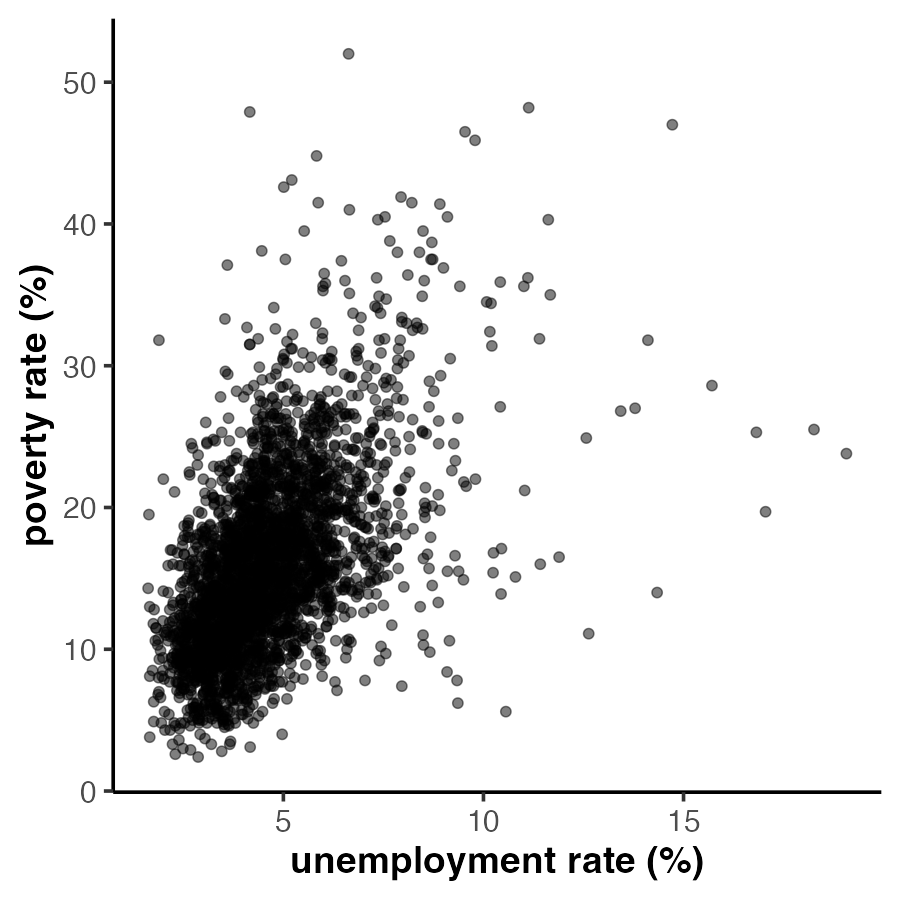
\includegraphics[width=\textwidth]{figures/unemployment-vs-poverty.png}
\end{center}
}

\end{frame}


%%%%%%%%%%%%%%%%%%%%%%%%%%%%%%%%%%%%

\subsection{Activity: reading scatterplots}

%%%%%%%%%%%%%%%%%%%%%%%%%%%%%%%%%%%%

\begin{frame}
\frametitle{Activity 2}

\twocol{0.5}{0.5}
{
\activity[-- reading scatterplots]{%
For each of the plots A--D, describe:
\begin{itemize}\setlength{\itemsep}{2pt}
\item direction,
\item form,
\item strength,
\item unusual observations.
\end{itemize}}
}
{
\begin{center}
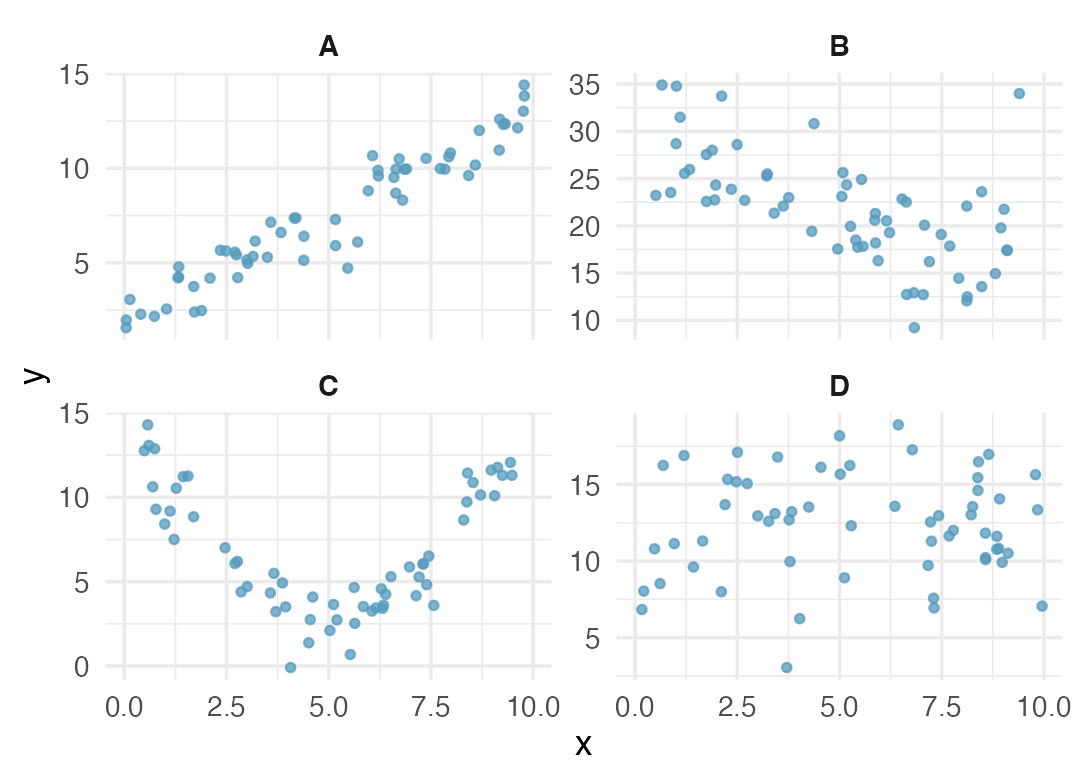
\includegraphics[width=\textwidth]{figures/lecture3_scatter_panels.png}
\end{center}
}
\end{frame}

%%%%%%%%%%%%%%%%%%%%%%%%%%%%%%%%%%%%

\begin{frame}
\frametitle{Activity 2}

\twocol{0.5}{0.5}
{
\solnbox{%
\textbf{A:} positive, linear, strong.\\
\textbf{B:} negative, linear, moderate, one clear outlier (top right).\\
\textbf{C:} nonlinear (U-shaped), strong.\\
\textbf{D:} no relationship.}

\vspace{0.4em}
When the form is linear, a straight line summarizes the trend. \hl{Next: write and fit that line.}
}
{
\begin{center}
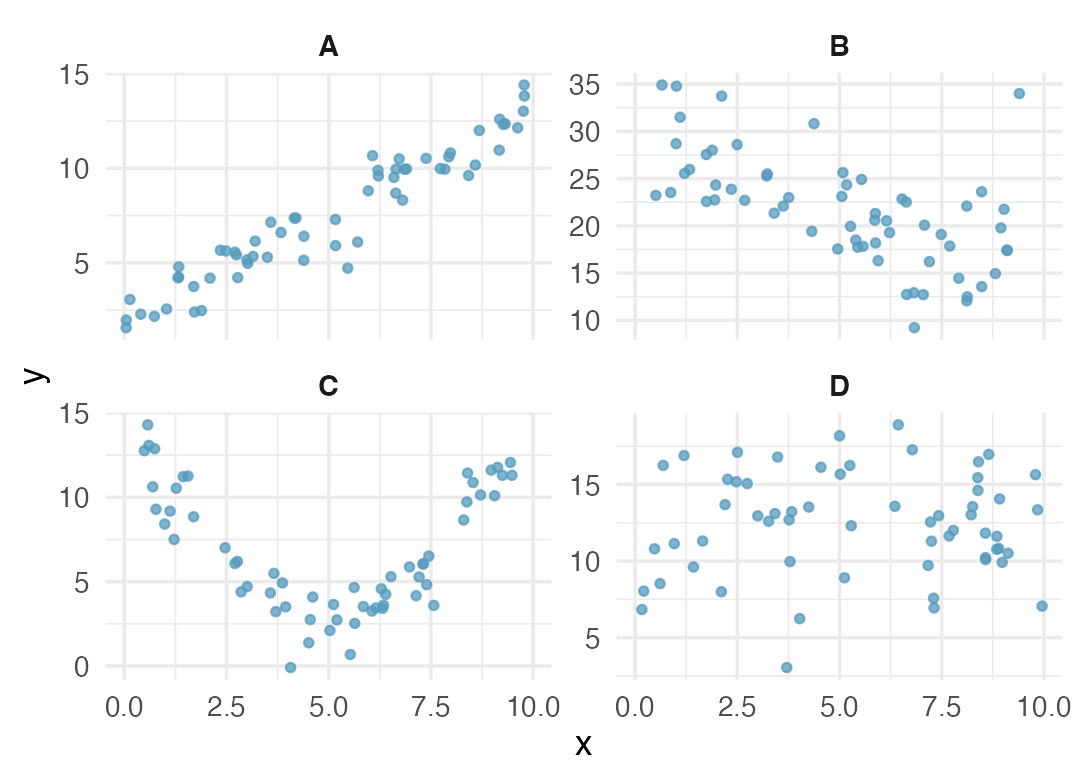
\includegraphics[width=\textwidth]{figures/lecture3_scatter_panels.png}
\end{center}
}
\end{frame}

%%%%%%%%%%%%%%%%%%%%%%%%%%%%%%%%%%%%
% Regression model
%%%%%%%%%%%%%%%%%%%%%%%%%%%%%%%%%%%%

\section{Simple linear regression model}

%%%%%%%%%%%%%%%%%%%%%%%%%%%%%%%%%%%%

\subsection{The model}

%%%%%%%%%%%%%%%%%%%%%%%%%%%%%%%%%%%%
\begin{frame}
\frametitle{A model for two variables}

For the county data, we want more than a picture:
\begin{itemize}
\item a \textbf{prediction} of poverty at any unemployment rate,
\item a description of the \textbf{scatter} around the trend.
\end{itemize}
A regression model provides both:

\begin{center}
\Large response = linear pattern + random error
\end{center}
\[
Y_i = \beta_0 + \beta_1 x_i + \varepsilon_i.
\]
\begin{itemize}
\item The line \(\beta_0 + \beta_1x_i\) describes the mean pattern.
\item The error term \(\varepsilon_i\) describes variation around the line.
\end{itemize}
\end{frame}


%%%%%%%%%%%%%%%%%%%%%%%%%%%%%%%%%%%%
\begin{frame}
\frametitle{A model for two variables}
        \begin{center}
		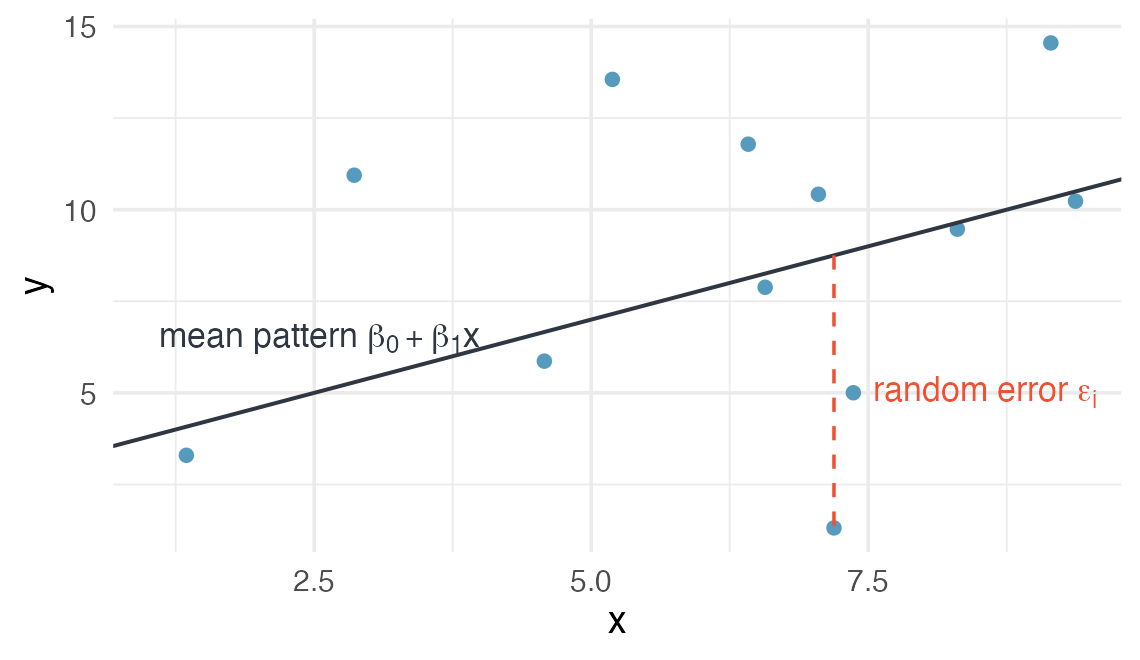
\includegraphics[width=1\textwidth]{figures/lecture3_model_decomposition.png}
		\end{center}

\end{frame}

%%%%%%%%%%%%%%%%%%%%%%%%%%%%%%%%%%%%

\begin{frame}
\frametitle{The simple linear regression model}

\formula{Simple linear regression model}{%
\[
Y_i = \beta_0 + \beta_1 x_i + \varepsilon_i
\]
\begin{itemize}
\item \(Y_i\): response variable for observation \(i\)
\item \(x_i\): explanatory variable value for observation \(i\)
\item \(\beta_0\): intercept parameter
\item \(\beta_1\): slope parameter
\item \(\varepsilon_i\): random error for observation \(i\)
\end{itemize}}

\end{frame}

%%%%%%%%%%%%%%%%%%%%%%%%%%%%%%%%%%%

\begin{frame}
\frametitle{Mean response}

If the random error has mean zero,
\[
E(\varepsilon_i)=0,
\]
then
\[
E(Y_i\mid x_i)=\beta_0+\beta_1x_i.
\]
\begin{itemize}
\item \(E(Y_i\mid x_i)\) reads ``the average value of \(Y_i\) among observations with explanatory value \(x_i\)'': the \hl{mean response} at \(x_i\).
\item Individual observations vary around this mean line.
\item The fitted line estimates this population mean line.
\end{itemize}

\end{frame}

%%%%%%%%%%%%%%%%%%%%%%%%%%%%%%%%%%%%

\begin{frame}
\frametitle{Model assumptions}

The simple linear regression model is \(Y_i=\beta_0+\beta_1x_i+\varepsilon_i\).
\formula{Model assumptions (LINE)}{%
\begin{itemize}
\item \textbf{L}inearity: the mean response is linear in \(x\).
\item \textbf{I}ndependent observations.
\item \textbf{N}ormal errors.
\item \textbf{E}qual variance: the spread around the line is constant.
\end{itemize}}
The normal-error assumption is what connects least squares to maximum likelihood.

\end{frame}
%%%%%%%%%%%%%%%%%%%%%%%%%%%%%%%%%%%%

\begin{frame}{Activity 3}
\activity[-- model assumptions]{%
\textbf{Worksheet Part 2:} for the model $Y_i=\beta_0+\beta_1x_i+\varepsilon_i$, match each LINE assumption to a short interpretation, in your own words.}
\end{frame}


%%%%%%%%%%%%%%%%%%%%%%%%%%%%%%%%%%%%

\begin{frame}
\frametitle{Population line and fitted line}

The population regression line is
\[
E(Y\mid x)=\beta_0+\beta_1x.
\]
Since \(\beta_0\) and \(\beta_1\) are unknown, we estimate them from data.


The fitted regression line is
\[
\widehat{y}
=
\widehat{\beta}_0+\widehat{\beta}_1x.
\]
\begin{itemize}
\item \(\beta_0,\beta_1\): unknown parameters.
\item \(\widehat{\beta}_0,\widehat{\beta}_1\): estimates from the data.
\end{itemize}
\end{frame}
%%%%%%%%%%%%%%%%%%%%%%%%%%%%%%%%%%%%
\begin{frame}
\frametitle{Population line and fitted line}
    \begin{center}
		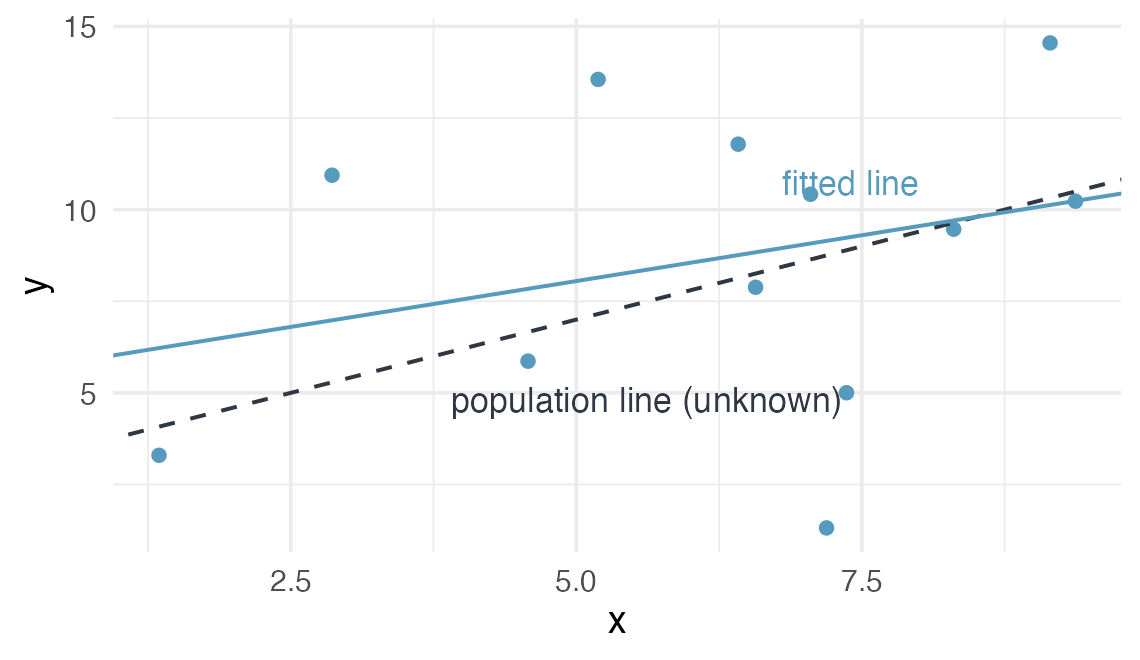
\includegraphics[width=1\textwidth]{figures/lecture3_population_vs_fitted.png}
		\end{center}

\end{frame}

%%%%%%%%%%%%%%%%%%%%%%%%%%%%%%%%%%%%
\subsection{Interpreting parameter estimates}
%%%%%%%%%%%%%%%%%%%%%%%%%%%%%%%%%%%%

\begin{frame}
\frametitle{Interpreting slope and intercept}

\twocol{0.5}{0.5}
{
\begin{itemize}
\item \hl{Intercept:} When \(x=0\), \(y\) is predicted to equal the intercept.

\vspace{0.8em}

\item \hl{Slope:} For each one-unit increase in \(x\), \(y\) is predicted to increase or decrease by the slope, on average --- an association, not necessarily a causal effect.
\end{itemize}
}
{
\begin{center}
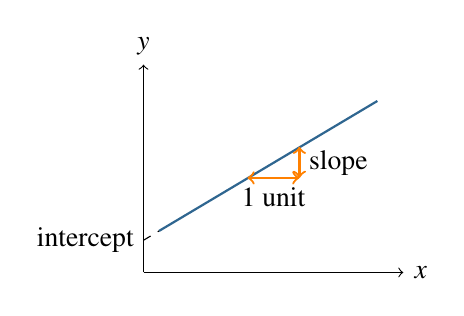
\begin{tikzpicture}[scale=0.66]
\draw[->] (0,0) -- (5,0) node[right] {$x$};
\draw[->] (0,0) -- (0,4) node[above] {$y$};
\draw[thick, oiB] (0.3,0.8) -- (4.5,3.3);
\draw[dashed] (0,0.62) -- (0.3,0.8);
\node[left] at (0,0.62) {intercept};
\draw[<->, orange, thick] (2.0,1.82) -- (3.0,1.82);
\draw[<->, orange, thick] (3.0,1.82) -- (3.0,2.42);
\node[below] at (2.5,1.82) {$1$ unit};
\node[right] at (3.0,2.1) {slope};
\end{tikzpicture}
\end{center}
}

\end{frame}

%%%%%%%%%%%%%%%%%%%%%%%%%%%%%%%%%%%%

\begin{frame}
\frametitle{Interpreting parameter estimates: Slope}
\examplehead{Unemployment and poverty}
The fitted county model is
\[
\widehat{\mathrm{poverty}} = 6.15 + 2.13 \times \mathrm{unemployment}.
\]
\hl{Interpretation:} For each additional percentage point of unemployment, the predicted poverty rate \emph{increases} by \(2.13\) percentage points, on average.

\end{frame}

%%%%%%%%%%%%%%%%%%%%%%%%%%%%%%%%%%%%

\begin{frame}
\frametitle{Interpreting parameter estimates: Intercept}
\examplehead{Unemployment and poverty}

The intercept \(\widehat{\beta}_0\) is the predicted response when \(x=0\).

\twocol{0.5}{0.5}
{
Here \(\widehat{\beta}_0 = 6.15\).

\hl{Interpretation:} a county with \(0\%\) unemployment is predicted to have a poverty rate of \(6.15\%\).

\vspace{0.2em}
\caution{Unemployment runs \(1.6\%\)--\(19\%\), so \(x=0\) is outside the data: the prediction is unreliable.}
}
{
\begin{center}
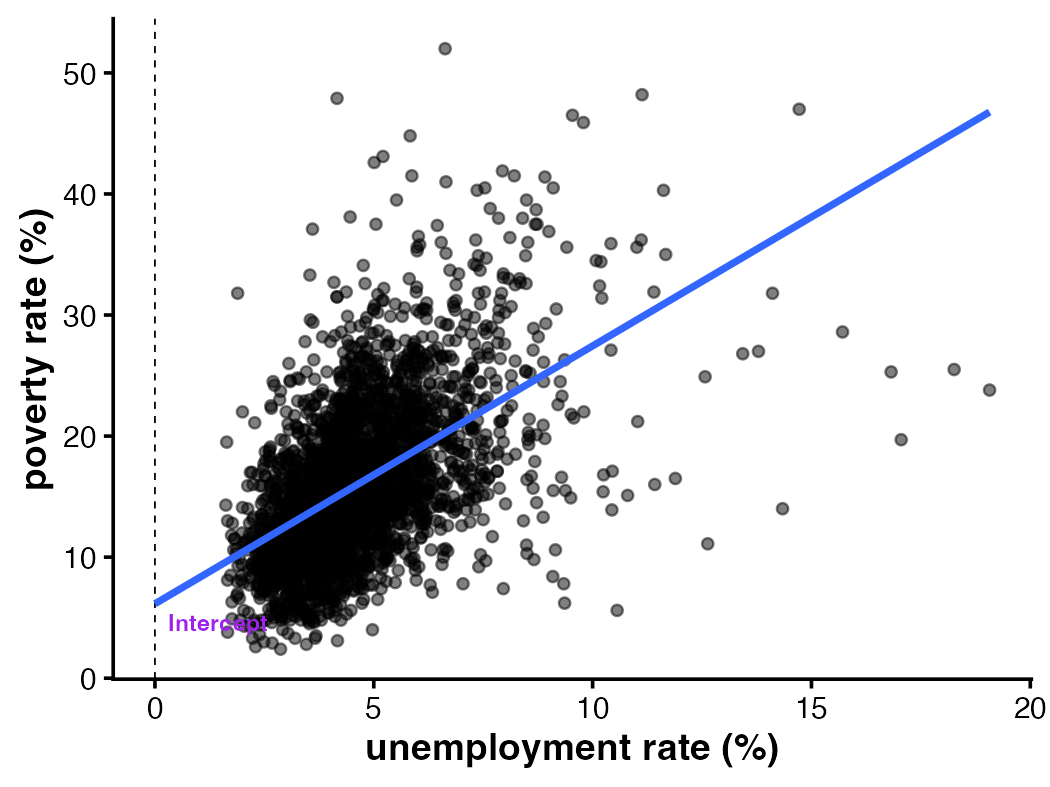
\includegraphics[width=0.85\textwidth]{figures/unemployment-vs-poverty-with-intercept.png}
\end{center}
}

\end{frame}

%%%%%%%%%%%%%%%%%%%%%%%%%%%%%%%%%%%%

\begin{frame}
\frametitle{Activity 4}
\examplehead{Unemployment and poverty}
\activity[-- apply the fitted line]{Use the fitted county model
\[
\widehat{\mathrm{poverty}} = 6.15 + 2.13 \times \mathrm{unemployment}.
\]
\begin{enumerate}
\item What does the ``hat'' on \(\widehat{\mathrm{poverty}}\) mean?
\item Predict the poverty rate for a county with a \(5\%\) unemployment rate.
\item Does this fitted line prove that lowering unemployment \emph{causes} lower poverty? Explain.
\end{enumerate}}

\end{frame}

%%%%%%%%%%%%%%%%%%%%%%%%%%%%%%%%%%%%

\begin{frame}
\frametitle{Activity 4}
\examplehead{Unemployment and poverty}
\begin{enumerate}
\item \soln{The ``hat'' marks a predicted (fitted) value from the model, not an observed data point.}

\pause

\item Prediction:
\[
\widehat{\mathrm{poverty}} = 6.15 + 2.13(5) = 16.8.
\]
\soln{The predicted poverty rate is about \(16.8\%\).}

\pause

\item \soln{No. These are observational county data, so the line shows association, not causation --- other factors (local industry, education, cost of living) can drive both variables.}
\end{enumerate}

\end{frame}
%%%%%%%%%%%%%%%%%%%%%%%%%%%%%%%%%%%%

\begin{frame}{Activity 5}
\activity[-- interpret and use fitted lines]{%
\textbf{Worksheet Parts 3--4:} two fitted models,
\[
\widehat{\text{rent}} = 800 + 2.5\times \text{size},
\qquad
\widehat{\text{score}} = 52 + 4.8\times \text{hours}.
\]
\begin{enumerate}
\item Identify the response and explanatory variables.
\item Interpret each slope and intercept in context.
\item Predict rent at $700$ sq ft and the score after $6$ study hours.
\end{enumerate}}
\end{frame}


%%%%%%%%%%%%%%%%%%%%%%%%%%%%%%%%%%%%

\section{Residuals}

%%%%%%%%%%%%%%%%%%%%%%%%%%%%%%%%%%%%

\begin{frame}
\frametitle{Residuals}
\examplehead{Unemployment and poverty}
\hl{Residuals} are the leftovers from the model fit: \(\text{Data} = \text{Fit} + \text{Residual}.\)

\twocol{0.5}{0.5}
{
\formula{Residual}{The residual for observation \(i\) is \; \(e_i = y_i - \widehat{y}_i\).}
\begin{itemize}
\item \textbf{Positive}: point \emph{above} the line (Jefferson County, MS).
\item \textbf{Negative}: point \emph{below} the line (Colusa County, CA).
\end{itemize}
}
{
\begin{center}
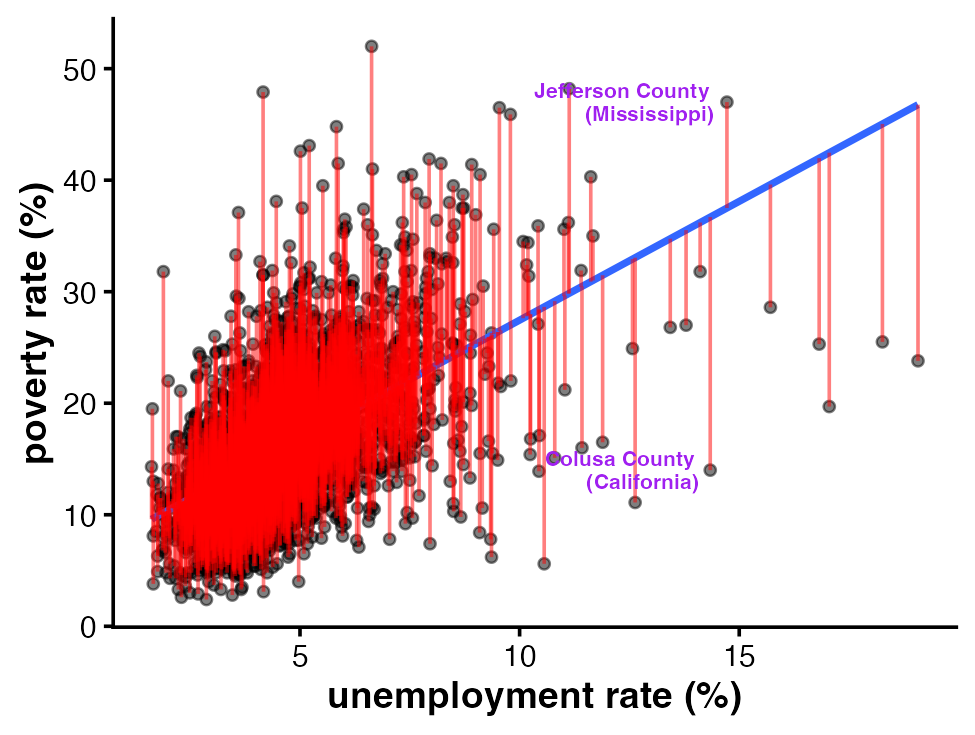
\includegraphics[width=0.78\textwidth]{figures/unemployment-vs-poverty-residuals-labeled.png}
\end{center}
}

\end{frame}

%%%%%%%%%%%%%%%%%%%%%%%%%%%%%%%%%%%%
\section{From maximum likelihood to least squares}
%%%%%%%%%%%%%%%%%%%%%%%%%%%%%%%%%%%%
\begin{frame}
\frametitle{Regression as a normal model}
For regression, assume the errors are normal:
\[
Y_i=\beta_0+\beta_1x_i+\varepsilon_i,
\qquad
\varepsilon_i\sim N(0,\sigma^2) \\
\Longleftrightarrow \qquad
Y_i\mid x_i \sim N(\beta_0+\beta_1x_i,\sigma^2).
\]
\begin{itemize}
\item The mean depends on \(x_i\); the variance \(\sigma^2\) describes spread around the line.
\item The parameters are \(\beta_0\), \(\beta_1\), and \(\sigma^2\).
\end{itemize}
\textbf{Fitting a line is now an MLE problem: choose the parameters that make the observed data most likely.}
\end{frame}
%%%%%%%%%%%%%%%%%%%%%%%%%%%%%%%%%%%%
\begin{frame}
\frametitle{Regression likelihood}

If
\[
Y_i\mid x_i \sim N(\beta_0+\beta_1x_i,\sigma^2),
\]
then the likelihood is
\[
L(\beta_0,\beta_1,\sigma^2)
=
\prod_{i=1}^{n}
\frac{1}{\sqrt{2\pi\sigma^2}}
\exp\left(
-\frac{(y_i-\beta_0-\beta_1x_i)^2}{2\sigma^2}
\right).
\]
The key term is the squared residual
\[
(y_i-\beta_0-\beta_1x_i)^2.
\]
\end{frame}
%%%%%%%%%%%%%%%%%%%%%%%%%%%%%%%%%%%%

\begin{frame}
\frametitle{Regression log-likelihood}

Taking logs gives
\[
\ell(\beta_0,\beta_1,\sigma^2)
=
-\frac{n}{2}\log(2\pi)
-\frac{n}{2}\log(\sigma^2)
-\frac{1}{2\sigma^2}
\sum_{i=1}^{n}
(y_i-\beta_0-\beta_1x_i)^2.
\]
For fixed \(\sigma^2\), maximizing this log-likelihood over \(\beta_0\) and \(\beta_1\) is the same as minimizing
\[
\sum_{i=1}^{n}
(y_i-\beta_0-\beta_1x_i)^2.
\]
So the most likely line is the one that minimizes this sum of squared residuals.

\end{frame}

%%%%%%%%%%%%%%%%%%%%%%%%%%%%%%%%%%%%

\begin{frame}
\frametitle{Residual sum of squares}
For any candidate line, the \hl{residual sum of squares} adds up the squared residuals:
\[
\operatorname{RSS}(\beta_0,\beta_1)=\sum_{i=1}^n (y_i-\beta_0-\beta_1x_i)^2.
\]
At the fitted line this equals \(\sum_{i=1}^n e_i^2\) --- the total squared vertical distance from the points to the line.
\end{frame}

%%%%%%%%%%%%%%%%%%%%%%%%%%%%%%%%%%%%

\begin{frame}
\frametitle{The least squares estimates}
The \hl{least squares estimates} are the candidate values that make the RSS smallest:
\formula{Least squares estimates}{%
\[
(\widehat{\beta}_0,\widehat{\beta}_1)
=
\operatorname*{arg\,min}_{\beta_0,\beta_1}
\sum_{i=1}^n
(y_i-\beta_0-\beta_1x_i)^2.
\]
\(\operatorname*{arg\,min}\) returns the \emph{values} of \(\beta_0,\beta_1\) that make the RSS smallest.}
\end{frame}

%%%%%%%%%%%%%%%%%%%%%%%%%%%%%%%%%%%%
\begin{frame}
\frametitle{Least squares as maximum likelihood}

The least squares estimates are
\[
(\widehat{\beta}_0,\widehat{\beta}_1)
=
\operatorname*{arg\,min}_{\beta_0,\beta_1}
\sum_{i=1}^{n}
(y_i-\beta_0-\beta_1x_i)^2.
\]
The maximum likelihood estimates are
\[
(\widehat{\beta}_0,\widehat{\beta}_1)
=
\operatorname*{arg\,max}_{\beta_0,\beta_1}
\ell(\beta_0,\beta_1,\sigma^2).
\]
\keyidea[-- Least squares = maximum likelihood]{Under the normal error model, the least squares line is the maximum likelihood line.}

\end{frame}

%%%%%%%%%%%%%%%%%%%%%%%%%%%%%%%%%%%%
\begin{frame}
\frametitle{Activity 6}

Compare two candidate lines for the data \((1,2),\ (2,4),\ (3,4)\):
\[
\text{Line A: } \hat y=1+x,
\qquad
\text{Line B: } \hat y=2+0.5x.
\]
\activity[-- which line is more likely?]{%
\textbf{Worksheet Part 5:} answer the same questions for the data set given there.
\begin{enumerate}
\item Compute the residuals for each line.
\item Compute the RSS for each line.
\item Under the same normal error model, which line gives the larger likelihood? 
\end{enumerate}}

\end{frame}





%%%%%%%%%%%%%%%%%%%%%%%%%%%%%%%%%%%%
% End document
%%%%%%%%%%%%%%%%%%%%%%%%%%%%%%%%%%%%

\end{document}
